\documentclass[1p]{elsarticle_modified}
%\bibliographystyle{elsarticle-num}

%\usepackage[colorlinks]{hyperref}
%\usepackage{abbrmath_seonhwa} %\Abb, \Ascr, \Acal ,\Abf, \Afrak
\usepackage{amsfonts}
\usepackage{amssymb}
\usepackage{amsmath}
\usepackage{amsthm}
\usepackage{scalefnt}
\usepackage{amsbsy}
\usepackage{kotex}
\usepackage{caption}
\usepackage{subfig}
\usepackage{color}
\usepackage{graphicx}
\usepackage{xcolor} %% white, black, red, green, blue, cyan, magenta, yellow
\usepackage{float}
\usepackage{setspace}
\usepackage{hyperref}

\usepackage{tikz}
\usetikzlibrary{arrows}

\usepackage{multirow}
\usepackage{array} % fixed length table
\usepackage{hhline}

%%%%%%%%%%%%%%%%%%%%%
\makeatletter
\renewcommand*\env@matrix[1][\arraystretch]{%
	\edef\arraystretch{#1}%
	\hskip -\arraycolsep
	\let\@ifnextchar\new@ifnextchar
	\array{*\c@MaxMatrixCols c}}
\makeatother %https://tex.stackexchange.com/questions/14071/how-can-i-increase-the-line-spacing-in-a-matrix
%%%%%%%%%%%%%%%

\usepackage[normalem]{ulem}

\newcommand{\msout}[1]{\ifmmode\text{\sout{\ensuremath{#1}}}\else\sout{#1}\fi}
%SOURCE: \msout is \stkout macro in https://tex.stackexchange.com/questions/20609/strikeout-in-math-mode

\newcommand{\cancel}[1]{
	\ifmmode
	{\color{red}\msout{#1}}
	\else
	{\color{red}\sout{#1}}
	\fi
}

\newcommand{\add}[1]{
	{\color{blue}\uwave{#1}}
}

\newcommand{\replace}[2]{
	\ifmmode
	{\color{red}\msout{#1}}{\color{blue}\uwave{#2}}
	\else
	{\color{red}\sout{#1}}{\color{blue}\uwave{#2}}
	\fi
}

\newcommand{\Sol}{\mathcal{S}} %segment
\newcommand{\D}{D} %diagram
\newcommand{\A}{\mathcal{A}} %arc


%%%%%%%%%%%%%%%%%%%%%%%%%%%%%5 test

\def\sl{\operatorname{\textup{SL}}(2,\Cbb)}
\def\psl{\operatorname{\textup{PSL}}(2,\Cbb)}
\def\quan{\mkern 1mu \triangleright \mkern 1mu}

\theoremstyle{definition}
\newtheorem{thm}{Theorem}[section]
\newtheorem{prop}[thm]{Proposition}
\newtheorem{lem}[thm]{Lemma}
\newtheorem{ques}[thm]{Question}
\newtheorem{cor}[thm]{Corollary}
\newtheorem{defn}[thm]{Definition}
\newtheorem{exam}[thm]{Example}
\newtheorem{rmk}[thm]{Remark}
\newtheorem{alg}[thm]{Algorithm}

\newcommand{\I}{\sqrt{-1}}
\begin{document}

%\begin{frontmatter}
%
%\title{Boundary parabolic representations of knots up to 8 crossings}
%
%%% Group authors per affiliation:
%\author{Yunhi Cho} 
%\address{Department of Mathematics, University of Seoul, Seoul, Korea}
%\ead{yhcho@uos.ac.kr}
%
%
%\author{Seonhwa Kim} %\fnref{s_kim}}
%\address{Center for Geometry and Physics, Institute for Basic Science, Pohang, 37673, Korea}
%\ead{ryeona17@ibs.re.kr}
%
%\author{Hyuk Kim}
%\address{Department of Mathematical Sciences, Seoul National University, Seoul 08826, Korea}
%\ead{hyukkim@snu.ac.kr}
%
%\author{Seokbeom Yoon}
%\address{Department of Mathematical Sciences, Seoul National University, Seoul, 08826,  Korea}
%\ead{sbyoon15@snu.ac.kr}
%
%\begin{abstract}
%We find all boundary parabolic representation of knots up to 8 crossings.
%
%\end{abstract}
%\begin{keyword}
%    \MSC[2010] 57M25 
%\end{keyword}
%
%\end{frontmatter}

%\linenumbers
%\tableofcontents
%
\newcommand\colored[1]{\textcolor{white}{\rule[-0.35ex]{0.8em}{1.4ex}}\kern-0.8em\color{red} #1}%
%\newcommand\colored[1]{\textcolor{white}{ #1}\kern-2.17ex	\textcolor{white}{ #1}\kern-1.81ex	\textcolor{white}{ #1}\kern-2.15ex\color{red}#1	}

{\Large $\underline{12n_{0414}~(K12n_{0414})}$}

\setlength{\tabcolsep}{10pt}
\renewcommand{\arraystretch}{1.6}
\vspace{1cm}\begin{tabular}{m{100pt}>{\centering\arraybackslash}m{274pt}}
\multirow{5}{120pt}{
	\centering
	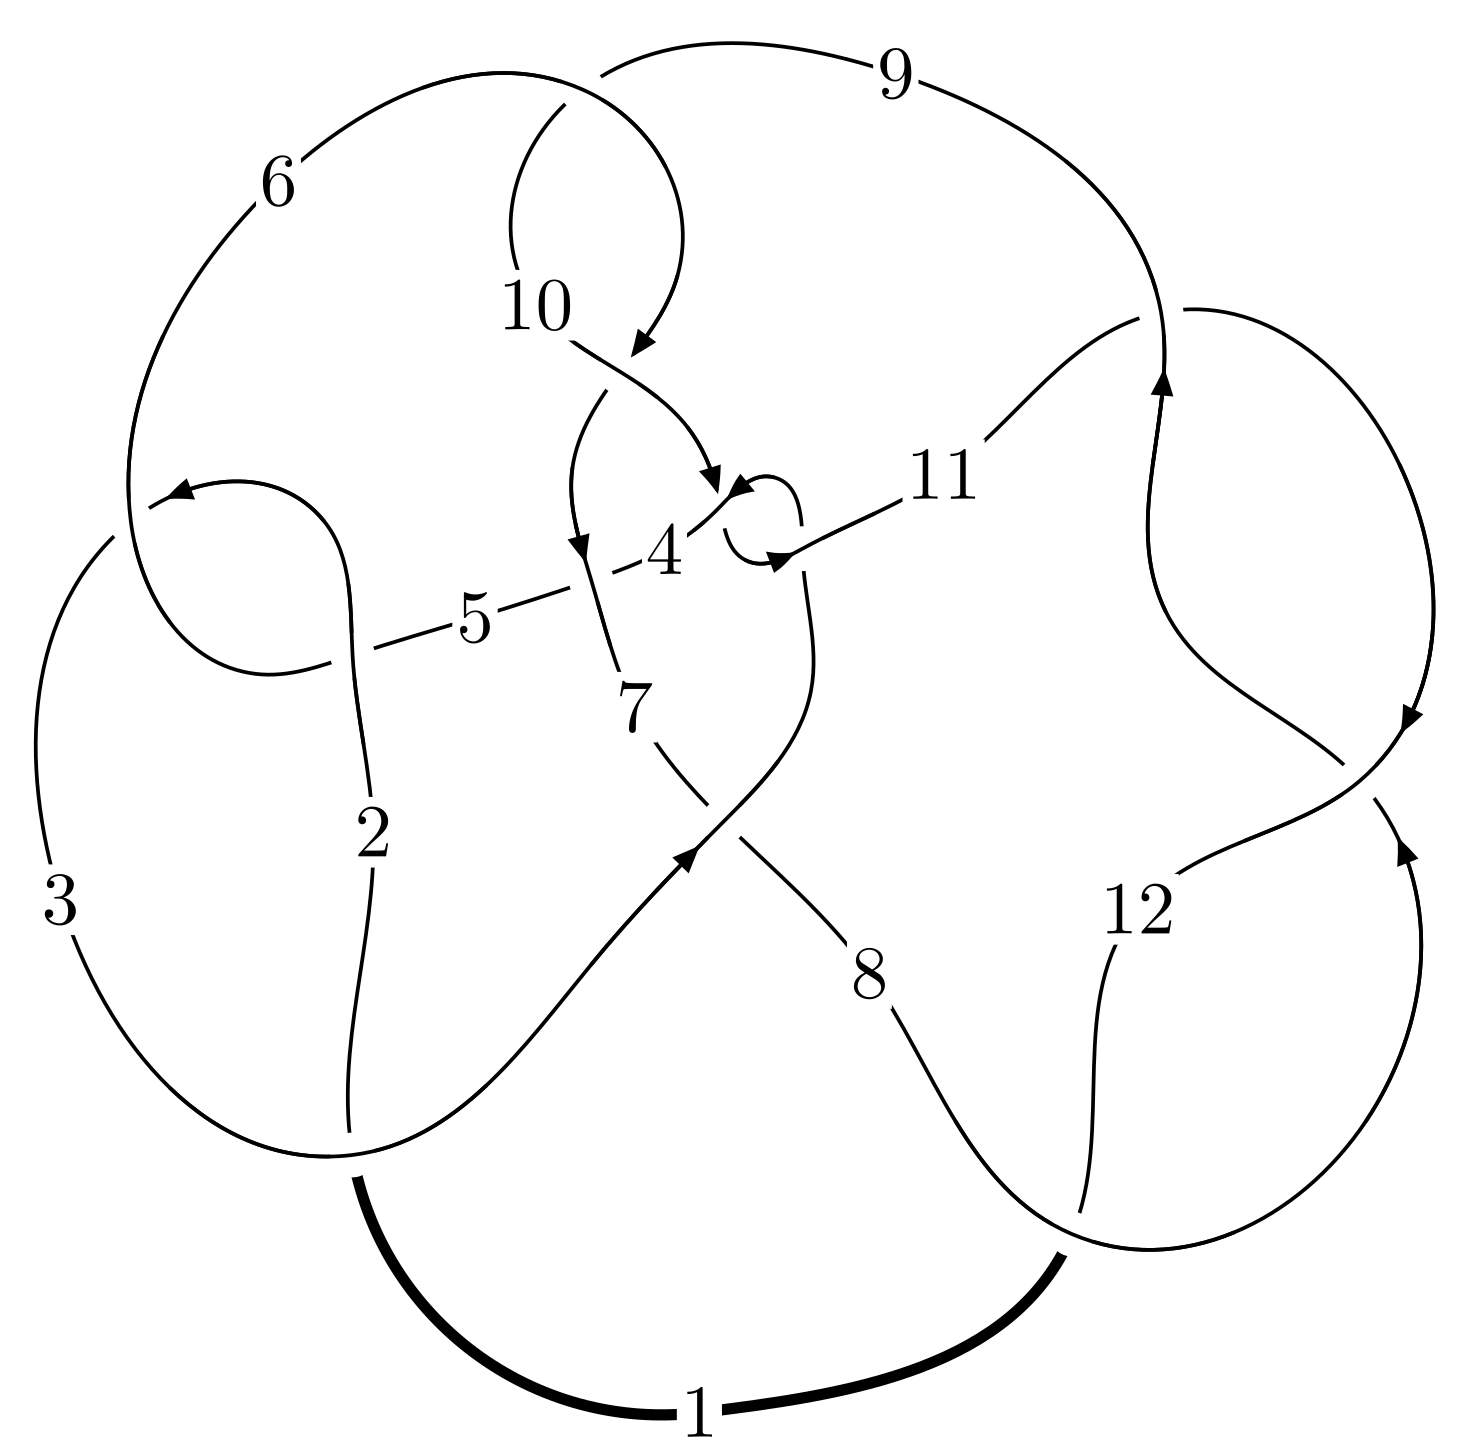
\includegraphics[width=112pt]{../../../GIT/diagram.site/Diagrams/png/2503_12n_0414.png}\\
\ \ \ A knot diagram\footnotemark}&
\allowdisplaybreaks
\textbf{Linearized knot diagam} \\
\cline{2-2}
 &
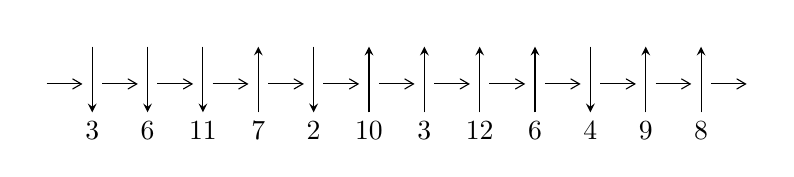
\begin{tikzpicture}[x=20pt, y=17pt]
	% nodes
	\node (C0) at (0, 0) {};
	\node (C1) at (1, 0) {};
	\node (C1U) at (1, +1) {};
	\node (C1D) at (1, -1) {3};

	\node (C2) at (2, 0) {};
	\node (C2U) at (2, +1) {};
	\node (C2D) at (2, -1) {6};

	\node (C3) at (3, 0) {};
	\node (C3U) at (3, +1) {};
	\node (C3D) at (3, -1) {11};

	\node (C4) at (4, 0) {};
	\node (C4U) at (4, +1) {};
	\node (C4D) at (4, -1) {7};

	\node (C5) at (5, 0) {};
	\node (C5U) at (5, +1) {};
	\node (C5D) at (5, -1) {2};

	\node (C6) at (6, 0) {};
	\node (C6U) at (6, +1) {};
	\node (C6D) at (6, -1) {10};

	\node (C7) at (7, 0) {};
	\node (C7U) at (7, +1) {};
	\node (C7D) at (7, -1) {3};

	\node (C8) at (8, 0) {};
	\node (C8U) at (8, +1) {};
	\node (C8D) at (8, -1) {12};

	\node (C9) at (9, 0) {};
	\node (C9U) at (9, +1) {};
	\node (C9D) at (9, -1) {6};

	\node (C10) at (10, 0) {};
	\node (C10U) at (10, +1) {};
	\node (C10D) at (10, -1) {4};

	\node (C11) at (11, 0) {};
	\node (C11U) at (11, +1) {};
	\node (C11D) at (11, -1) {9};

	\node (C12) at (12, 0) {};
	\node (C12U) at (12, +1) {};
	\node (C12D) at (12, -1) {8};
	\node (C13) at (13, 0) {};

	% arrows
	\draw[->,>={angle 60}]
	(C0) edge (C1) (C1) edge (C2) (C2) edge (C3) (C3) edge (C4) (C4) edge (C5) (C5) edge (C6) (C6) edge (C7) (C7) edge (C8) (C8) edge (C9) (C9) edge (C10) (C10) edge (C11) (C11) edge (C12) (C12) edge (C13) ;	\draw[->,>=stealth]
	(C1U) edge (C1D) (C2U) edge (C2D) (C3U) edge (C3D) (C4D) edge (C4U) (C5U) edge (C5D) (C6D) edge (C6U) (C7D) edge (C7U) (C8D) edge (C8U) (C9D) edge (C9U) (C10U) edge (C10D) (C11D) edge (C11U) (C12D) edge (C12U) ;
	\end{tikzpicture} \\
\hhline{~~} \\& 
\textbf{Solving Sequence} \\ \cline{2-2} 
 &
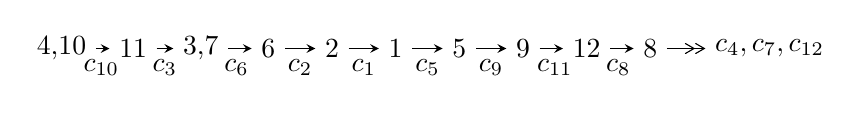
\begin{tikzpicture}[x=23pt, y=7pt]
	% node
	\node (A0) at (-1/8, 0) {4,10};
	\node (A1) at (1, 0) {11};
	\node (A2) at (33/16, 0) {3,7};
	\node (A3) at (25/8, 0) {6};
	\node (A4) at (33/8, 0) {2};
	\node (A5) at (41/8, 0) {1};
	\node (A6) at (49/8, 0) {5};
	\node (A7) at (57/8, 0) {9};
	\node (A8) at (65/8, 0) {12};
	\node (A9) at (73/8, 0) {8};
	\node (C1) at (1/2, -1) {$c_{10}$};
	\node (C2) at (3/2, -1) {$c_{3}$};
	\node (C3) at (21/8, -1) {$c_{6}$};
	\node (C4) at (29/8, -1) {$c_{2}$};
	\node (C5) at (37/8, -1) {$c_{1}$};
	\node (C6) at (45/8, -1) {$c_{5}$};
	\node (C7) at (53/8, -1) {$c_{9}$};
	\node (C8) at (61/8, -1) {$c_{11}$};
	\node (C9) at (69/8, -1) {$c_{8}$};
	\node (A10) at (11, 0) {$c_{4},c_{7},c_{12}$};

	% edge
	\draw[->,>=stealth]	
	(A0) edge (A1) (A1) edge (A2) (A2) edge (A3) (A3) edge (A4) (A4) edge (A5) (A5) edge (A6) (A6) edge (A7) (A7) edge (A8) (A8) edge (A9) ;
	\draw[->>,>={angle 60}]	
	(A9) edge (A10);
\end{tikzpicture} \\ 

\end{tabular} \\

\footnotetext{
The image of knot diagram is generated by the software ``\textbf{Draw programme}" developed by Andrew Bartholomew(\url{http://www.layer8.co.uk/maths/draw/index.htm\#Running-draw}), where we modified some parts for our purpose(\url{https://github.com/CATsTAILs/LinksPainter}).
}\phantom \\ \newline 
\centering \textbf{Ideals for irreducible components\footnotemark of $X_{\text{par}}$} 
 
\begin{align*}
I^u_{1}&=\langle 
- u^{14}-6 u^{13}+\cdots+2 b+6,\;-5 u^{14}-28 u^{13}+\cdots+4 a+20,\;u^{15}+6 u^{14}+\cdots-10 u-4\rangle \\
I^u_{2}&=\langle 
- u^{10}- u^9-5 u^8-4 u^7-9 u^6-5 u^5-6 u^4+b+2 u+1,\;- u^9-4 u^7-5 u^5-2 u^3+u^2+a- u+1,\\
\phantom{I^u_{2}}&\phantom{= \langle  }u^{11}+u^{10}+6 u^9+5 u^8+13 u^7+8 u^6+11 u^5+2 u^4+u^3-4 u^2-2 u-1\rangle \\
I^u_{3}&=\langle 
b- u+1,\;a^2-5 a u+a+u-4,\;u^2- u+1\rangle \\
I^u_{4}&=\langle 
b+u,\;a^2+3 a u+2 u,\;u^2- u+1\rangle \\
\\
\end{align*}
\raggedright * 4 irreducible components of $\dim_{\mathbb{C}}=0$, with total 34 representations.\\
\footnotetext{All coefficients of polynomials are rational numbers. But the coefficients are sometimes approximated in decimal forms when there is not enough margin.}
\newpage
\renewcommand{\arraystretch}{1}
\centering \section*{I. $I^u_{1}= \langle - u^{14}-6 u^{13}+\cdots+2 b+6,\;-5 u^{14}-28 u^{13}+\cdots+4 a+20,\;u^{15}+6 u^{14}+\cdots-10 u-4 \rangle$}
\flushleft \textbf{(i) Arc colorings}\\
\begin{tabular}{m{7pt} m{180pt} m{7pt} m{180pt} }
\flushright $a_{4}=$&$\begin{pmatrix}0\\u\end{pmatrix}$ \\
\flushright $a_{10}=$&$\begin{pmatrix}1\\0\end{pmatrix}$ \\
\flushright $a_{11}=$&$\begin{pmatrix}1\\u^2\end{pmatrix}$ \\
\flushright $a_{3}=$&$\begin{pmatrix}u\\u^3+u\end{pmatrix}$ \\
\flushright $a_{7}=$&$\begin{pmatrix}\frac{5}{4} u^{14}+7 u^{13}+\cdots-\frac{29}{4} u-5\\\frac{1}{2} u^{14}+3 u^{13}+\cdots-\frac{7}{2} u-3\end{pmatrix}$ \\
\flushright $a_{6}=$&$\begin{pmatrix}\frac{3}{4} u^{14}+4 u^{13}+\cdots-\frac{15}{4} u-2\\\frac{1}{2} u^{14}+3 u^{13}+\cdots-\frac{7}{2} u-3\end{pmatrix}$ \\
\flushright $a_{2}=$&$\begin{pmatrix}-\frac{1}{2} u^{13}-2 u^{12}+\cdots+\frac{5}{2} u+\frac{3}{2}\\\frac{1}{2} u^{14}+2 u^{13}+\cdots-\frac{1}{2} u^2-\frac{1}{2} u\end{pmatrix}$ \\
\flushright $a_{1}=$&$\begin{pmatrix}-\frac{1}{2} u^{13}-4 u^{12}+\cdots+\frac{11}{2} u+\frac{7}{2}\\-\frac{3}{2} u^{14}-5 u^{13}+\cdots+\frac{5}{2} u+2\end{pmatrix}$ \\
\flushright $a_{5}=$&$\begin{pmatrix}-\frac{3}{2} u^{14}-\frac{17}{2} u^{13}+\cdots+12 u+\frac{15}{2}\\-\frac{1}{2} u^{14}-3 u^{13}+\cdots+\frac{15}{2} u+4\end{pmatrix}$ \\
\flushright $a_{9}=$&$\begin{pmatrix}\frac{1}{2} u^{14}+\frac{5}{2} u^{13}+\cdots- u-\frac{1}{2}\\\frac{1}{2} u^{14}+3 u^{13}+\cdots-\frac{7}{2} u-2\end{pmatrix}$ \\
\flushright $a_{12}=$&$\begin{pmatrix}\frac{1}{4} u^{14}+u^{13}+\cdots-\frac{1}{4} u+1\\-\frac{1}{2} u^{14}-2 u^{13}+\cdots+\frac{1}{2} u+1\end{pmatrix}$ \\
\flushright $a_{8}=$&$\begin{pmatrix}-\frac{7}{4} u^{14}-8 u^{13}+\cdots+\frac{19}{4} u+1\\-\frac{5}{2} u^{14}-15 u^{13}+\cdots+\frac{53}{2} u+15\end{pmatrix}$\\&\end{tabular}
\flushleft \textbf{(ii) Obstruction class $= -1$}\\~\\
\flushleft \textbf{(iii) Cusp Shapes $= u^{14}+6 u^{13}+24 u^{12}+69 u^{11}+155 u^{10}+287 u^9+438 u^8+568 u^7+616 u^6+556 u^5+409 u^4+223 u^3+82 u^2+4 u-10$}\\~\\
\newpage\renewcommand{\arraystretch}{1}
\flushleft \textbf{(iv) u-Polynomials at the component}\newline \\
\begin{tabular}{m{50pt}|m{274pt}}
Crossings & \hspace{64pt}u-Polynomials at each crossing \\
\hline $$\begin{aligned}c_{1}\end{aligned}$$&$\begin{aligned}
&u^{15}+30 u^{14}+\cdots+116 u+1
\end{aligned}$\\
\hline $$\begin{aligned}c_{2},c_{5}\end{aligned}$$&$\begin{aligned}
&u^{15}+2 u^{14}+\cdots+16 u-1
\end{aligned}$\\
\hline $$\begin{aligned}c_{3},c_{10}\end{aligned}$$&$\begin{aligned}
&u^{15}+6 u^{14}+\cdots-10 u-4
\end{aligned}$\\
\hline $$\begin{aligned}c_{4}\end{aligned}$$&$\begin{aligned}
&u^{15}+3 u^{14}+\cdots+147 u-167
\end{aligned}$\\
\hline $$\begin{aligned}c_{6},c_{9}\end{aligned}$$&$\begin{aligned}
&u^{15}-8 u^{14}+\cdots+10 u-4
\end{aligned}$\\
\hline $$\begin{aligned}c_{7}\end{aligned}$$&$\begin{aligned}
&u^{15}- u^{14}+\cdots+504 u-821
\end{aligned}$\\
\hline $$\begin{aligned}c_{8},c_{11},c_{12}\end{aligned}$$&$\begin{aligned}
&u^{15}+12 u^{13}+\cdots+2 u-1
\end{aligned}$\\
\hline
\end{tabular}\\~\\
\newpage\renewcommand{\arraystretch}{1}
\flushleft \textbf{(v) Riley Polynomials at the component}\newline \\
\begin{tabular}{m{50pt}|m{274pt}}
Crossings & \hspace{64pt}Riley Polynomials at each crossing \\
\hline $$\begin{aligned}c_{1}\end{aligned}$$&$\begin{aligned}
&y^{15}-126 y^{14}+\cdots+10676 y-1
\end{aligned}$\\
\hline $$\begin{aligned}c_{2},c_{5}\end{aligned}$$&$\begin{aligned}
&y^{15}-30 y^{14}+\cdots+116 y-1
\end{aligned}$\\
\hline $$\begin{aligned}c_{3},c_{10}\end{aligned}$$&$\begin{aligned}
&y^{15}+12 y^{14}+\cdots+172 y-16
\end{aligned}$\\
\hline $$\begin{aligned}c_{4}\end{aligned}$$&$\begin{aligned}
&y^{15}+7 y^{14}+\cdots+36973 y-27889
\end{aligned}$\\
\hline $$\begin{aligned}c_{6},c_{9}\end{aligned}$$&$\begin{aligned}
&y^{15}-2 y^{14}+\cdots-20 y-16
\end{aligned}$\\
\hline $$\begin{aligned}c_{7}\end{aligned}$$&$\begin{aligned}
&y^{15}+93 y^{14}+\cdots+6938598 y-674041
\end{aligned}$\\
\hline $$\begin{aligned}c_{8},c_{11},c_{12}\end{aligned}$$&$\begin{aligned}
&y^{15}+24 y^{14}+\cdots-4 y-1
\end{aligned}$\\
\hline
\end{tabular}\\~\\
\newpage\flushleft \textbf{(vi) Complex Volumes and Cusp Shapes}
$$\begin{array}{c|c|c}  
\text{Solutions to }I^u_{1}& \I (\text{vol} + \sqrt{-1}CS) & \text{Cusp shape}\\
 \hline 
\begin{aligned}
u &= -0.155852 + 1.083570 I \\
a &= \phantom{-}0.034406 + 0.857462 I \\
b &= \phantom{-}0.175953 + 0.734858 I\end{aligned}
 & \phantom{-}1.28315 + 1.86492 I & \phantom{-}2.71830 - 4.33042 I \\ \hline\begin{aligned}
u &= -0.155852 - 1.083570 I \\
a &= \phantom{-}0.034406 - 0.857462 I \\
b &= \phantom{-}0.175953 - 0.734858 I\end{aligned}
 & \phantom{-}1.28315 - 1.86492 I & \phantom{-}2.71830 + 4.33042 I \\ \hline\begin{aligned}
u &= \phantom{-}0.259042 + 1.188320 I \\
a &= -0.462640 - 1.221370 I \\
b &= \phantom{-}1.117260 - 0.423512 I\end{aligned}
 & \phantom{-}4.14035 - 2.21303 I & \phantom{-}4.08061 - 1.06114 I \\ \hline\begin{aligned}
u &= \phantom{-}0.259042 - 1.188320 I \\
a &= -0.462640 + 1.221370 I \\
b &= \phantom{-}1.117260 + 0.423512 I\end{aligned}
 & \phantom{-}4.14035 + 2.21303 I & \phantom{-}4.08061 + 1.06114 I \\ \hline\begin{aligned}
u &= -1.222820 + 0.037634 I \\
a &= \phantom{-}0.85572 - 1.76718 I \\
b &= \phantom{-}1.14186 - 1.14785 I\end{aligned}
 & \phantom{-}18.7646 - 4.2382 I & -2.01730 + 1.87492 I \\ \hline\begin{aligned}
u &= -1.222820 - 0.037634 I \\
a &= \phantom{-}0.85572 + 1.76718 I \\
b &= \phantom{-}1.14186 + 1.14785 I\end{aligned}
 & \phantom{-}18.7646 + 4.2382 I & -2.01730 - 1.87492 I \\ \hline\begin{aligned}
u &= -0.598605 + 0.209178 I \\
a &= \phantom{-}0.372970 - 1.207580 I \\
b &= -0.361721 - 0.520276 I\end{aligned}
 & -1.20899 + 0.97971 I & -3.43147 - 3.17255 I \\ \hline\begin{aligned}
u &= -0.598605 - 0.209178 I \\
a &= \phantom{-}0.372970 + 1.207580 I \\
b &= -0.361721 + 0.520276 I\end{aligned}
 & -1.20899 - 0.97971 I & -3.43147 + 3.17255 I \\ \hline\begin{aligned}
u &= -0.229749 + 1.394560 I \\
a &= \phantom{-}0.797940 - 0.746930 I \\
b &= -0.762956 - 0.521556 I\end{aligned}
 & \phantom{-}3.94947 + 4.00013 I & \phantom{-}0.81375 - 5.52037 I \\ \hline\begin{aligned}
u &= -0.229749 - 1.394560 I \\
a &= \phantom{-}0.797940 + 0.746930 I \\
b &= -0.762956 + 0.521556 I\end{aligned}
 & \phantom{-}3.94947 - 4.00013 I & \phantom{-}0.81375 + 5.52037 I\\
 \hline 
 \end{array}$$\newpage$$\begin{array}{c|c|c}  
\text{Solutions to }I^u_{1}& \I (\text{vol} + \sqrt{-1}CS) & \text{Cusp shape}\\
 \hline 
\begin{aligned}
u &= -0.62184 + 1.42460 I \\
a &= -0.48987 + 1.78057 I \\
b &= \phantom{-}1.09118 + 1.20044 I\end{aligned}
 & -16.3948 + 10.7667 I & \phantom{-}0.20728 - 4.66775 I \\ \hline\begin{aligned}
u &= -0.62184 - 1.42460 I \\
a &= -0.48987 - 1.78057 I \\
b &= \phantom{-}1.09118 - 1.20044 I\end{aligned}
 & -16.3948 - 10.7667 I & \phantom{-}0.20728 + 4.66775 I \\ \hline\begin{aligned}
u &= -0.58488 + 1.47267 I \\
a &= \phantom{-}0.767227 - 0.411092 I \\
b &= \phantom{-}1.21709 - 1.11271 I\end{aligned}
 & -15.9766 + 2.2090 I & \phantom{-}0.250029 - 0.743127 I \\ \hline\begin{aligned}
u &= -0.58488 - 1.47267 I \\
a &= \phantom{-}0.767227 + 0.411092 I \\
b &= \phantom{-}1.21709 + 1.11271 I\end{aligned}
 & -15.9766 - 2.2090 I & \phantom{-}0.250029 + 0.743127 I \\ \hline\begin{aligned}
u &= \phantom{-}0.309403\phantom{ +0.000000I} \\
a &= \phantom{-}1.74849\phantom{ +0.000000I} \\
b &= \phantom{-}0.762664\phantom{ +0.000000I}\end{aligned}
 & \phantom{-}1.01627\phantom{ +0.000000I} & \phantom{-}11.7580\phantom{ +0.000000I}\\
 \hline 
 \end{array}$$\newpage\newpage\renewcommand{\arraystretch}{1}
\centering \section*{II. $I^u_{2}= \langle - u^{10}- u^9+\cdots+b+1,\;- u^9-4 u^7-5 u^5-2 u^3+u^2+a- u+1,\;u^{11}+u^{10}+\cdots-2 u-1 \rangle$}
\flushleft \textbf{(i) Arc colorings}\\
\begin{tabular}{m{7pt} m{180pt} m{7pt} m{180pt} }
\flushright $a_{4}=$&$\begin{pmatrix}0\\u\end{pmatrix}$ \\
\flushright $a_{10}=$&$\begin{pmatrix}1\\0\end{pmatrix}$ \\
\flushright $a_{11}=$&$\begin{pmatrix}1\\u^2\end{pmatrix}$ \\
\flushright $a_{3}=$&$\begin{pmatrix}u\\u^3+u\end{pmatrix}$ \\
\flushright $a_{7}=$&$\begin{pmatrix}u^9+4 u^7+5 u^5+2 u^3- u^2+u-1\\u^{10}+u^9+5 u^8+4 u^7+9 u^6+5 u^5+6 u^4-2 u-1\end{pmatrix}$ \\
\flushright $a_{6}=$&$\begin{pmatrix}- u^{10}-5 u^8-9 u^6-6 u^4+2 u^3- u^2+3 u\\u^{10}+u^9+5 u^8+4 u^7+9 u^6+5 u^5+6 u^4-2 u-1\end{pmatrix}$ \\
\flushright $a_{2}=$&$\begin{pmatrix}u^{10}+u^9+6 u^8+4 u^7+12 u^6+4 u^5+8 u^4-2 u^3- u^2-3 u\\- u^8- u^7-4 u^6-3 u^5-5 u^4- u^3- u^2+3 u+1\end{pmatrix}$ \\
\flushright $a_{1}=$&$\begin{pmatrix}- u^9+u^8-4 u^7+4 u^6-5 u^5+5 u^4-2 u^3+2 u^2-2 u+1\\u^{10}+u^9+4 u^8+3 u^7+4 u^6+u^5-2 u^4-3 u^3-3 u^2+u+1\end{pmatrix}$ \\
\flushright $a_{5}=$&$\begin{pmatrix}- u^{10}-2 u^9-6 u^8-9 u^7-12 u^6-13 u^5-7 u^4-3 u^3+4 u^2+4 u+2\\- u^{10}- u^9-5 u^8-4 u^7-8 u^6-4 u^5-3 u^4+2 u^3+2 u^2+3 u\end{pmatrix}$ \\
\flushright $a_{9}=$&$\begin{pmatrix}u^{10}+u^9+5 u^8+3 u^7+8 u^6+u^5+3 u^4-4 u^3- u^2-2 u+2\\- u^{10}-2 u^9-6 u^8-8 u^7-12 u^6-9 u^5-7 u^4+u^3+3 u^2+4 u+1\end{pmatrix}$ \\
\flushright $a_{12}=$&$\begin{pmatrix}2 u^{10}+3 u^9+12 u^8+14 u^7+25 u^6+20 u^5+18 u^4+3 u^3-3 u^2-9 u-3\\- u^9- u^8-5 u^7-4 u^6-8 u^5-4 u^4-4 u^3+3 u^2+u+2\end{pmatrix}$ \\
\flushright $a_{8}=$&$\begin{pmatrix}-2 u^{10}- u^9-9 u^8-3 u^7-13 u^6- u^5-4 u^4+5 u^3+2 u^2+3 u-1\\2 u^{10}+2 u^9+9 u^8+7 u^7+14 u^6+6 u^5+7 u^4-3 u^3- u^2-2 u-1\end{pmatrix}$\\&\end{tabular}
\flushleft \textbf{(ii) Obstruction class $= 1$}\\~\\
\flushleft \textbf{(iii) Cusp Shapes $= 2 u^{10}+u^9+9 u^8+4 u^7+16 u^6+4 u^5+12 u^4-5 u^3+u^2-7 u-1$}\\~\\
\newpage\renewcommand{\arraystretch}{1}
\flushleft \textbf{(iv) u-Polynomials at the component}\newline \\
\begin{tabular}{m{50pt}|m{274pt}}
Crossings & \hspace{64pt}u-Polynomials at each crossing \\
\hline $$\begin{aligned}c_{1}\end{aligned}$$&$\begin{aligned}
&u^{11}-8 u^{10}+\cdots+6 u-1
\end{aligned}$\\
\hline $$\begin{aligned}c_{2}\end{aligned}$$&$\begin{aligned}
&u^{11}+2 u^{10}-2 u^9-5 u^8+2 u^7+6 u^6- u^5-5 u^4+u^3+3 u^2-1
\end{aligned}$\\
\hline $$\begin{aligned}c_{3}\end{aligned}$$&$\begin{aligned}
&u^{11}- u^{10}+6 u^9-5 u^8+13 u^7-8 u^6+11 u^5-2 u^4+u^3+4 u^2-2 u+1
\end{aligned}$\\
\hline $$\begin{aligned}c_{4}\end{aligned}$$&$\begin{aligned}
&u^{11}+3 u^{10}+\cdots+5 u+1
\end{aligned}$\\
\hline $$\begin{aligned}c_{5}\end{aligned}$$&$\begin{aligned}
&u^{11}-2 u^{10}-2 u^9+5 u^8+2 u^7-6 u^6- u^5+5 u^4+u^3-3 u^2+1
\end{aligned}$\\
\hline $$\begin{aligned}c_{6}\end{aligned}$$&$\begin{aligned}
&u^{11}-3 u^{10}+3 u^9+2 u^8-8 u^7+7 u^6+3 u^5-9 u^4+5 u^3+2 u^2-3 u+1
\end{aligned}$\\
\hline $$\begin{aligned}c_{7}\end{aligned}$$&$\begin{aligned}
&u^{11}+u^{10}+\cdots+20 u^2-1
\end{aligned}$\\
\hline $$\begin{aligned}c_{8}\end{aligned}$$&$\begin{aligned}
&u^{11}+7 u^9- u^8+19 u^7-4 u^6+24 u^5-5 u^4+12 u^3- u^2+1
\end{aligned}$\\
\hline $$\begin{aligned}c_{9}\end{aligned}$$&$\begin{aligned}
&u^{11}+3 u^{10}+3 u^9-2 u^8-8 u^7-7 u^6+3 u^5+9 u^4+5 u^3-2 u^2-3 u-1
\end{aligned}$\\
\hline $$\begin{aligned}c_{10}\end{aligned}$$&$\begin{aligned}
&u^{11}+u^{10}+6 u^9+5 u^8+13 u^7+8 u^6+11 u^5+2 u^4+u^3-4 u^2-2 u-1
\end{aligned}$\\
\hline $$\begin{aligned}c_{11},c_{12}\end{aligned}$$&$\begin{aligned}
&u^{11}+7 u^9+u^8+19 u^7+4 u^6+24 u^5+5 u^4+12 u^3+u^2-1
\end{aligned}$\\
\hline
\end{tabular}\\~\\
\newpage\renewcommand{\arraystretch}{1}
\flushleft \textbf{(v) Riley Polynomials at the component}\newline \\
\begin{tabular}{m{50pt}|m{274pt}}
Crossings & \hspace{64pt}Riley Polynomials at each crossing \\
\hline $$\begin{aligned}c_{1}\end{aligned}$$&$\begin{aligned}
&y^{11}-8 y^{10}+\cdots-2 y-1
\end{aligned}$\\
\hline $$\begin{aligned}c_{2},c_{5}\end{aligned}$$&$\begin{aligned}
&y^{11}-8 y^{10}+\cdots+6 y-1
\end{aligned}$\\
\hline $$\begin{aligned}c_{3},c_{10}\end{aligned}$$&$\begin{aligned}
&y^{11}+11 y^{10}+\cdots-4 y-1
\end{aligned}$\\
\hline $$\begin{aligned}c_{4}\end{aligned}$$&$\begin{aligned}
&y^{11}-3 y^{10}+\cdots- y-1
\end{aligned}$\\
\hline $$\begin{aligned}c_{6},c_{9}\end{aligned}$$&$\begin{aligned}
&y^{11}-3 y^{10}+\cdots+5 y-1
\end{aligned}$\\
\hline $$\begin{aligned}c_{7}\end{aligned}$$&$\begin{aligned}
&y^{11}-13 y^{10}+\cdots+40 y-1
\end{aligned}$\\
\hline $$\begin{aligned}c_{8},c_{11},c_{12}\end{aligned}$$&$\begin{aligned}
&y^{11}+14 y^{10}+\cdots+2 y-1
\end{aligned}$\\
\hline
\end{tabular}\\~\\
\newpage\flushleft \textbf{(vi) Complex Volumes and Cusp Shapes}
$$\begin{array}{c|c|c}  
\text{Solutions to }I^u_{2}& \I (\text{vol} + \sqrt{-1}CS) & \text{Cusp shape}\\
 \hline 
\begin{aligned}
u &= -0.555245 + 0.715930 I \\
a &= -1.365260 - 0.336962 I \\
b &= -0.541266 - 0.326647 I\end{aligned}
 & -4.78843 + 2.37248 I & -1.75049 - 2.45336 I \\ \hline\begin{aligned}
u &= -0.555245 - 0.715930 I \\
a &= -1.365260 + 0.336962 I \\
b &= -0.541266 + 0.326647 I\end{aligned}
 & -4.78843 - 2.37248 I & -1.75049 + 2.45336 I \\ \hline\begin{aligned}
u &= -0.038740 + 1.275640 I \\
a &= \phantom{-}0.634053 + 1.055000 I \\
b &= -0.481027 + 1.188790 I\end{aligned}
 & -1.63477 - 1.57892 I & \phantom{-}0.09382 + 1.50767 I \\ \hline\begin{aligned}
u &= -0.038740 - 1.275640 I \\
a &= \phantom{-}0.634053 - 1.055000 I \\
b &= -0.481027 - 1.188790 I\end{aligned}
 & -1.63477 + 1.57892 I & \phantom{-}0.09382 - 1.50767 I \\ \hline\begin{aligned}
u &= \phantom{-}0.671399\phantom{ +0.000000I} \\
a &= \phantom{-}0.781778\phantom{ +0.000000I} \\
b &= \phantom{-}0.881691\phantom{ +0.000000I}\end{aligned}
 & \phantom{-}0.262796\phantom{ +0.000000I} & -1.63010\phantom{ +0.000000I} \\ \hline\begin{aligned}
u &= \phantom{-}0.261659 + 1.352930 I \\
a &= -0.528351 - 0.791252 I \\
b &= \phantom{-}0.983118 - 0.233645 I\end{aligned}
 & \phantom{-}4.64860 - 3.37974 I & \phantom{-}7.26008 + 1.85613 I \\ \hline\begin{aligned}
u &= \phantom{-}0.261659 - 1.352930 I \\
a &= -0.528351 + 0.791252 I \\
b &= \phantom{-}0.983118 + 0.233645 I\end{aligned}
 & \phantom{-}4.64860 + 3.37974 I & \phantom{-}7.26008 - 1.85613 I \\ \hline\begin{aligned}
u &= -0.20259 + 1.44175 I \\
a &= \phantom{-}0.349549 - 0.489012 I \\
b &= -1.265600 - 0.591843 I\end{aligned}
 & \phantom{-}1.36871 + 4.84258 I & \phantom{-}1.85800 - 4.12088 I \\ \hline\begin{aligned}
u &= -0.20259 - 1.44175 I \\
a &= \phantom{-}0.349549 + 0.489012 I \\
b &= -1.265600 + 0.591843 I\end{aligned}
 & \phantom{-}1.36871 - 4.84258 I & \phantom{-}1.85800 + 4.12088 I \\ \hline\begin{aligned}
u &= -0.300781 + 0.431635 I \\
a &= -0.980876 + 0.585854 I \\
b &= -0.636073 - 0.679052 I\end{aligned}
 & -4.66031 + 2.37297 I & -0.14637 - 2.89222 I\\
 \hline 
 \end{array}$$\newpage$$\begin{array}{c|c|c}  
\text{Solutions to }I^u_{2}& \I (\text{vol} + \sqrt{-1}CS) & \text{Cusp shape}\\
 \hline 
\begin{aligned}
u &= -0.300781 - 0.431635 I \\
a &= -0.980876 - 0.585854 I \\
b &= -0.636073 + 0.679052 I\end{aligned}
 & -4.66031 - 2.37297 I & -0.14637 + 2.89222 I\\
 \hline 
 \end{array}$$\newpage\newpage\renewcommand{\arraystretch}{1}
\centering \section*{III. $I^u_{3}= \langle b- u+1,\;a^2-5 a u+a+u-4,\;u^2- u+1 \rangle$}
\flushleft \textbf{(i) Arc colorings}\\
\begin{tabular}{m{7pt} m{180pt} m{7pt} m{180pt} }
\flushright $a_{4}=$&$\begin{pmatrix}0\\u\end{pmatrix}$ \\
\flushright $a_{10}=$&$\begin{pmatrix}1\\0\end{pmatrix}$ \\
\flushright $a_{11}=$&$\begin{pmatrix}1\\u-1\end{pmatrix}$ \\
\flushright $a_{3}=$&$\begin{pmatrix}u\\u-1\end{pmatrix}$ \\
\flushright $a_{7}=$&$\begin{pmatrix}a\\u-1\end{pmatrix}$ \\
\flushright $a_{6}=$&$\begin{pmatrix}a- u+1\\u-1\end{pmatrix}$ \\
\flushright $a_{2}=$&$\begin{pmatrix}a u-3 a+4 u-1\\- a u+2 u-3\end{pmatrix}$ \\
\flushright $a_{1}=$&$\begin{pmatrix}2 a u-5 a+5 u-1\\-2 a u- a+3 u-4\end{pmatrix}$ \\
\flushright $a_{5}=$&$\begin{pmatrix}4 a u-5 a+3 u+1\\- a+u\end{pmatrix}$ \\
\flushright $a_{9}=$&$\begin{pmatrix}a u- a+u+1\\- u\end{pmatrix}$ \\
\flushright $a_{12}=$&$\begin{pmatrix}a u+u+1\\a u- a+u+1\end{pmatrix}$ \\
\flushright $a_{8}=$&$\begin{pmatrix}2 a- u\\a u\end{pmatrix}$\\&\end{tabular}
\flushleft \textbf{(ii) Obstruction class $= -1$}\\~\\
\flushleft \textbf{(iii) Cusp Shapes $= 8 u-6$}\\~\\
\newpage\renewcommand{\arraystretch}{1}
\flushleft \textbf{(iv) u-Polynomials at the component}\newline \\
\begin{tabular}{m{50pt}|m{274pt}}
Crossings & \hspace{64pt}u-Polynomials at each crossing \\
\hline $$\begin{aligned}c_{1}\end{aligned}$$&$\begin{aligned}
&u^4+11 u^3+45 u^2+44 u+16
\end{aligned}$\\
\hline $$\begin{aligned}c_{2},c_{5}\end{aligned}$$&$\begin{aligned}
&u^4+3 u^3- u^2-6 u+4
\end{aligned}$\\
\hline $$\begin{aligned}c_{3},c_{10}\end{aligned}$$&$\begin{aligned}
&(u^2- u+1)^2
\end{aligned}$\\
\hline $$\begin{aligned}c_{4}\end{aligned}$$&$\begin{aligned}
&u^4+6 u^3+23 u^2+30 u+13
\end{aligned}$\\
\hline $$\begin{aligned}c_{6},c_{9}\end{aligned}$$&$\begin{aligned}
&(u^2+u+1)^2
\end{aligned}$\\
\hline $$\begin{aligned}c_{7}\end{aligned}$$&$\begin{aligned}
&u^4+5 u^3+5 u^2-2 u+4
\end{aligned}$\\
\hline $$\begin{aligned}c_{8},c_{11},c_{12}\end{aligned}$$&$\begin{aligned}
&u^4+2 u^3+5 u^2+4 u+7
\end{aligned}$\\
\hline
\end{tabular}\\~\\
\newpage\renewcommand{\arraystretch}{1}
\flushleft \textbf{(v) Riley Polynomials at the component}\newline \\
\begin{tabular}{m{50pt}|m{274pt}}
Crossings & \hspace{64pt}Riley Polynomials at each crossing \\
\hline $$\begin{aligned}c_{1}\end{aligned}$$&$\begin{aligned}
&y^4-31 y^3+1089 y^2-496 y+256
\end{aligned}$\\
\hline $$\begin{aligned}c_{2},c_{5}\end{aligned}$$&$\begin{aligned}
&y^4-11 y^3+45 y^2-44 y+16
\end{aligned}$\\
\hline $$\begin{aligned}c_{3},c_{6},c_{9}\\c_{10}\end{aligned}$$&$\begin{aligned}
&(y^2+y+1)^2
\end{aligned}$\\
\hline $$\begin{aligned}c_{4}\end{aligned}$$&$\begin{aligned}
&y^4+10 y^3+195 y^2-302 y+169
\end{aligned}$\\
\hline $$\begin{aligned}c_{7}\end{aligned}$$&$\begin{aligned}
&y^4-15 y^3+53 y^2+36 y+16
\end{aligned}$\\
\hline $$\begin{aligned}c_{8},c_{11},c_{12}\end{aligned}$$&$\begin{aligned}
&y^4+6 y^3+23 y^2+54 y+49
\end{aligned}$\\
\hline
\end{tabular}\\~\\
\newpage\flushleft \textbf{(vi) Complex Volumes and Cusp Shapes}
$$\begin{array}{c|c|c}  
\text{Solutions to }I^u_{3}& \I (\text{vol} + \sqrt{-1}CS) & \text{Cusp shape}\\
 \hline 
\begin{aligned}
u &= \phantom{-}0.500000 + 0.866025 I \\
a &= -0.208440 + 0.922644 I \\
b &= -0.500000 + 0.866025 I\end{aligned}
 & -4.93480 - 4.05977 I & -2.00000 + 6.92820 I \\ \hline\begin{aligned}
u &= \phantom{-}0.500000 + 0.866025 I \\
a &= \phantom{-}1.70844 + 3.40748 I \\
b &= -0.500000 + 0.866025 I\end{aligned}
 & -4.93480 - 4.05977 I & -2.00000 + 6.92820 I \\ \hline\begin{aligned}
u &= \phantom{-}0.500000 - 0.866025 I \\
a &= -0.208440 - 0.922644 I \\
b &= -0.500000 - 0.866025 I\end{aligned}
 & -4.93480 + 4.05977 I & -2.00000 - 6.92820 I \\ \hline\begin{aligned}
u &= \phantom{-}0.500000 - 0.866025 I \\
a &= \phantom{-}1.70844 - 3.40748 I \\
b &= -0.500000 - 0.866025 I\end{aligned}
 & -4.93480 + 4.05977 I & -2.00000 - 6.92820 I\\
 \hline 
 \end{array}$$\newpage\newpage\renewcommand{\arraystretch}{1}
\centering \section*{IV. $I^u_{4}= \langle b+u,\;a^2+3 a u+2 u,\;u^2- u+1 \rangle$}
\flushleft \textbf{(i) Arc colorings}\\
\begin{tabular}{m{7pt} m{180pt} m{7pt} m{180pt} }
\flushright $a_{4}=$&$\begin{pmatrix}0\\u\end{pmatrix}$ \\
\flushright $a_{10}=$&$\begin{pmatrix}1\\0\end{pmatrix}$ \\
\flushright $a_{11}=$&$\begin{pmatrix}1\\u-1\end{pmatrix}$ \\
\flushright $a_{3}=$&$\begin{pmatrix}u\\u-1\end{pmatrix}$ \\
\flushright $a_{7}=$&$\begin{pmatrix}a\\- u\end{pmatrix}$ \\
\flushright $a_{6}=$&$\begin{pmatrix}a+u\\- u\end{pmatrix}$ \\
\flushright $a_{2}=$&$\begin{pmatrix}a u+1\\a+2 u\end{pmatrix}$ \\
\flushright $a_{1}=$&$\begin{pmatrix}3 a u- a\\a u- a+u\end{pmatrix}$ \\
\flushright $a_{5}=$&$\begin{pmatrix}-3 a u+3 a-2 u+2\\- a u+a+u\end{pmatrix}$ \\
\flushright $a_{9}=$&$\begin{pmatrix}- a u- u+2\\u-1\end{pmatrix}$ \\
\flushright $a_{12}=$&$\begin{pmatrix}a u+3 u\\a u- a+u-2\end{pmatrix}$ \\
\flushright $a_{8}=$&$\begin{pmatrix}2 a+1\\a u\end{pmatrix}$\\&\end{tabular}
\flushleft \textbf{(ii) Obstruction class $= -1$}\\~\\
\flushleft \textbf{(iii) Cusp Shapes $= -2$}\\~\\
\newpage\renewcommand{\arraystretch}{1}
\flushleft \textbf{(iv) u-Polynomials at the component}\newline \\
\begin{tabular}{m{50pt}|m{274pt}}
Crossings & \hspace{64pt}u-Polynomials at each crossing \\
\hline $$\begin{aligned}c_{1}\end{aligned}$$&$\begin{aligned}
&u^4+2 u^3+15 u^2+50 u+49
\end{aligned}$\\
\hline $$\begin{aligned}c_{2},c_{5}\end{aligned}$$&$\begin{aligned}
&u^4- u^2+6 u+7
\end{aligned}$\\
\hline $$\begin{aligned}c_{3},c_{10}\end{aligned}$$&$\begin{aligned}
&(u^2- u+1)^2
\end{aligned}$\\
\hline $$\begin{aligned}c_{4}\end{aligned}$$&$\begin{aligned}
&u^4-3 u^3+5 u^2+6 u+4
\end{aligned}$\\
\hline $$\begin{aligned}c_{6},c_{9}\end{aligned}$$&$\begin{aligned}
&(u^2+u+1)^2
\end{aligned}$\\
\hline $$\begin{aligned}c_{7}\end{aligned}$$&$\begin{aligned}
&u^4-4 u^3+5 u^2+4 u+1
\end{aligned}$\\
\hline $$\begin{aligned}c_{8},c_{11},c_{12}\end{aligned}$$&$\begin{aligned}
&u^4- u^3+5 u^2-2 u+4
\end{aligned}$\\
\hline
\end{tabular}\\~\\
\newpage\renewcommand{\arraystretch}{1}
\flushleft \textbf{(v) Riley Polynomials at the component}\newline \\
\begin{tabular}{m{50pt}|m{274pt}}
Crossings & \hspace{64pt}Riley Polynomials at each crossing \\
\hline $$\begin{aligned}c_{1}\end{aligned}$$&$\begin{aligned}
&y^4+26 y^3+123 y^2-1030 y+2401
\end{aligned}$\\
\hline $$\begin{aligned}c_{2},c_{5}\end{aligned}$$&$\begin{aligned}
&y^4-2 y^3+15 y^2-50 y+49
\end{aligned}$\\
\hline $$\begin{aligned}c_{3},c_{6},c_{9}\\c_{10}\end{aligned}$$&$\begin{aligned}
&(y^2+y+1)^2
\end{aligned}$\\
\hline $$\begin{aligned}c_{4}\end{aligned}$$&$\begin{aligned}
&y^4+y^3+69 y^2+4 y+16
\end{aligned}$\\
\hline $$\begin{aligned}c_{7}\end{aligned}$$&$\begin{aligned}
&y^4-6 y^3+59 y^2-6 y+1
\end{aligned}$\\
\hline $$\begin{aligned}c_{8},c_{11},c_{12}\end{aligned}$$&$\begin{aligned}
&y^4+9 y^3+29 y^2+36 y+16
\end{aligned}$\\
\hline
\end{tabular}\\~\\
\newpage\flushleft \textbf{(vi) Complex Volumes and Cusp Shapes}
$$\begin{array}{c|c|c}  
\text{Solutions to }I^u_{4}& \I (\text{vol} + \sqrt{-1}CS) & \text{Cusp shape}\\
 \hline 
\begin{aligned}
u &= \phantom{-}0.500000 + 0.866025 I \\
a &= -0.675835 + 0.160585 I \\
b &= -0.500000 - 0.866025 I\end{aligned}
 & -4.93480\phantom{ +0.000000I} & -2.00000\phantom{ +0.000000I} \\ \hline\begin{aligned}
u &= \phantom{-}0.500000 + 0.866025 I \\
a &= -0.82417 - 2.75866 I \\
b &= -0.500000 - 0.866025 I\end{aligned}
 & -4.93480\phantom{ +0.000000I} & -2.00000\phantom{ +0.000000I} \\ \hline\begin{aligned}
u &= \phantom{-}0.500000 - 0.866025 I \\
a &= -0.675835 - 0.160585 I \\
b &= -0.500000 + 0.866025 I\end{aligned}
 & -4.93480\phantom{ +0.000000I} & -2.00000\phantom{ +0.000000I} \\ \hline\begin{aligned}
u &= \phantom{-}0.500000 - 0.866025 I \\
a &= -0.82417 + 2.75866 I \\
b &= -0.500000 + 0.866025 I\end{aligned}
 & -4.93480\phantom{ +0.000000I} & -2.00000\phantom{ +0.000000I}\\
 \hline 
 \end{array}$$\newpage
\newpage\renewcommand{\arraystretch}{1}
\centering \section*{ V. u-Polynomials}
\begin{tabular}{m{50pt}|m{274pt}}
Crossings & \hspace{64pt}u-Polynomials at each crossing \\
\hline $$\begin{aligned}c_{1}\end{aligned}$$&$\begin{aligned}
&(u^4+2 u^3+15 u^2+50 u+49)(u^4+11 u^3+45 u^2+44 u+16)\\
&\cdot(u^{11}-8 u^{10}+\cdots+6 u-1)(u^{15}+30 u^{14}+\cdots+116 u+1)
\end{aligned}$\\
\hline $$\begin{aligned}c_{2}\end{aligned}$$&$\begin{aligned}
&(u^4- u^2+6 u+7)(u^4+3 u^3- u^2-6 u+4)\\
&\cdot(u^{11}+2 u^{10}-2 u^9-5 u^8+2 u^7+6 u^6- u^5-5 u^4+u^3+3 u^2-1)\\
&\cdot(u^{15}+2 u^{14}+\cdots+16 u-1)
\end{aligned}$\\
\hline $$\begin{aligned}c_{3}\end{aligned}$$&$\begin{aligned}
&(u^2- u+1)^4\\
&\cdot(u^{11}- u^{10}+6 u^9-5 u^8+13 u^7-8 u^6+11 u^5-2 u^4+u^3+4 u^2-2 u+1)\\
&\cdot(u^{15}+6 u^{14}+\cdots-10 u-4)
\end{aligned}$\\
\hline $$\begin{aligned}c_{4}\end{aligned}$$&$\begin{aligned}
&(u^4-3 u^3+5 u^2+6 u+4)(u^4+6 u^3+23 u^2+30 u+13)\\
&\cdot(u^{11}+3 u^{10}+\cdots+5 u+1)(u^{15}+3 u^{14}+\cdots+147 u-167)
\end{aligned}$\\
\hline $$\begin{aligned}c_{5}\end{aligned}$$&$\begin{aligned}
&(u^4- u^2+6 u+7)(u^4+3 u^3- u^2-6 u+4)\\
&\cdot(u^{11}-2 u^{10}-2 u^9+5 u^8+2 u^7-6 u^6- u^5+5 u^4+u^3-3 u^2+1)\\
&\cdot(u^{15}+2 u^{14}+\cdots+16 u-1)
\end{aligned}$\\
\hline $$\begin{aligned}c_{6}\end{aligned}$$&$\begin{aligned}
&(u^2+u+1)^4\\
&\cdot(u^{11}-3 u^{10}+3 u^9+2 u^8-8 u^7+7 u^6+3 u^5-9 u^4+5 u^3+2 u^2-3 u+1)\\
&\cdot(u^{15}-8 u^{14}+\cdots+10 u-4)
\end{aligned}$\\
\hline $$\begin{aligned}c_{7}\end{aligned}$$&$\begin{aligned}
&(u^4-4 u^3+5 u^2+4 u+1)(u^4+5 u^3+5 u^2-2 u+4)\\
&\cdot(u^{11}+u^{10}+\cdots+20 u^2-1)(u^{15}- u^{14}+\cdots+504 u-821)
\end{aligned}$\\
\hline $$\begin{aligned}c_{8}\end{aligned}$$&$\begin{aligned}
&(u^4- u^3+5 u^2-2 u+4)(u^4+2 u^3+5 u^2+4 u+7)\\
&\cdot(u^{11}+7 u^9- u^8+19 u^7-4 u^6+24 u^5-5 u^4+12 u^3- u^2+1)\\
&\cdot(u^{15}+12 u^{13}+\cdots+2 u-1)
\end{aligned}$\\
\hline $$\begin{aligned}c_{9}\end{aligned}$$&$\begin{aligned}
&(u^2+u+1)^4\\
&\cdot(u^{11}+3 u^{10}+3 u^9-2 u^8-8 u^7-7 u^6+3 u^5+9 u^4+5 u^3-2 u^2-3 u-1)\\
&\cdot(u^{15}-8 u^{14}+\cdots+10 u-4)
\end{aligned}$\\
\hline $$\begin{aligned}c_{10}\end{aligned}$$&$\begin{aligned}
&(u^2- u+1)^4\\
&\cdot(u^{11}+u^{10}+6 u^9+5 u^8+13 u^7+8 u^6+11 u^5+2 u^4+u^3-4 u^2-2 u-1)\\
&\cdot(u^{15}+6 u^{14}+\cdots-10 u-4)
\end{aligned}$\\
\hline $$\begin{aligned}c_{11},c_{12}\end{aligned}$$&$\begin{aligned}
&(u^4- u^3+5 u^2-2 u+4)(u^4+2 u^3+5 u^2+4 u+7)\\
&\cdot(u^{11}+7 u^9+u^8+19 u^7+4 u^6+24 u^5+5 u^4+12 u^3+u^2-1)\\
&\cdot(u^{15}+12 u^{13}+\cdots+2 u-1)
\end{aligned}$\\
\hline
\end{tabular}\newpage\renewcommand{\arraystretch}{1}
\centering \section*{ VI. Riley Polynomials}
\begin{tabular}{m{50pt}|m{274pt}}
Crossings & \hspace{64pt}Riley Polynomials at each crossing \\
\hline $$\begin{aligned}c_{1}\end{aligned}$$&$\begin{aligned}
&(y^4-31 y^3+1089 y^2-496 y+256)\\
&\cdot(y^4+26 y^3+\cdots-1030 y+2401)(y^{11}-8 y^{10}+\cdots-2 y-1)\\
&\cdot(y^{15}-126 y^{14}+\cdots+10676 y-1)
\end{aligned}$\\
\hline $$\begin{aligned}c_{2},c_{5}\end{aligned}$$&$\begin{aligned}
&(y^4-11 y^3+45 y^2-44 y+16)(y^4-2 y^3+15 y^2-50 y+49)\\
&\cdot(y^{11}-8 y^{10}+\cdots+6 y-1)(y^{15}-30 y^{14}+\cdots+116 y-1)
\end{aligned}$\\
\hline $$\begin{aligned}c_{3},c_{10}\end{aligned}$$&$\begin{aligned}
&((y^2+y+1)^4)(y^{11}+11 y^{10}+\cdots-4 y-1)\\
&\cdot(y^{15}+12 y^{14}+\cdots+172 y-16)
\end{aligned}$\\
\hline $$\begin{aligned}c_{4}\end{aligned}$$&$\begin{aligned}
&(y^4+y^3+69 y^2+4 y+16)(y^4+10 y^3+195 y^2-302 y+169)\\
&\cdot(y^{11}-3 y^{10}+\cdots- y-1)(y^{15}+7 y^{14}+\cdots+36973 y-27889)
\end{aligned}$\\
\hline $$\begin{aligned}c_{6},c_{9}\end{aligned}$$&$\begin{aligned}
&((y^2+y+1)^4)(y^{11}-3 y^{10}+\cdots+5 y-1)(y^{15}-2 y^{14}+\cdots-20 y-16)
\end{aligned}$\\
\hline $$\begin{aligned}c_{7}\end{aligned}$$&$\begin{aligned}
&(y^4-15 y^3+53 y^2+36 y+16)(y^4-6 y^3+59 y^2-6 y+1)\\
&\cdot(y^{11}-13 y^{10}+\cdots+40 y-1)\\
&\cdot(y^{15}+93 y^{14}+\cdots+6938598 y-674041)
\end{aligned}$\\
\hline $$\begin{aligned}c_{8},c_{11},c_{12}\end{aligned}$$&$\begin{aligned}
&(y^4+6 y^3+23 y^2+54 y+49)(y^4+9 y^3+29 y^2+36 y+16)\\
&\cdot(y^{11}+14 y^{10}+\cdots+2 y-1)(y^{15}+24 y^{14}+\cdots-4 y-1)
\end{aligned}$\\
\hline
\end{tabular}
\vskip 2pc
\end{document}